% -*- Mode:TeX -*-

%% IMPORTANT: The official thesis specifications are available at:
%%            http://libraries.mit.edu/archives/thesis-specs/
%%
%%            Please verify your thesis' formatting and copyright
%%            assignment before submission.  If you notice any
%%            discrepancies between these templates and the 
%%            MIT Libraries' specs, please let us know
%%            by e-mailing thesis@mit.edu

%% The documentclass options along with the pagestyle can be used to generate
%% a technical report, a draft copy, or a regular thesis.  You may need to
%% re-specify the pagestyle after you \include  cover.tex.  For more
%% information, see the first few lines of mitthesis.cls. 

%\documentclass[12pt,vi,twoside]{mitthesis}
%%
%%  If you want your thesis copyright to you instead of MIT, use the
%%  ``vi'' option, as above.
%%
%\documentclass[12pt,twoside,leftblank]{mitthesis}
%%
%% If you want blank pages before new chapters to be labelled ``This
%% Page Intentionally Left Blank'', use the ``leftblank'' option, as
%% above.

\documentclass[12pt,twoside]{mitthesis}
\usepackage{lgrind}
%% These have been added at the request of the MIT Libraries, because
%% some PDF conversions mess up the ligatures.  -LB, 1/22/2014
\usepackage{cmap}
\usepackage[T1]{fontenc}
\usepackage{hyperref}
\usepackage{listings}
\usepackage{xcolor}
\usepackage{graphicx}
\usepackage{amsfonts}
\usepackage{cleveref}
\usepackage{bytefield}
\usepackage[font=small,labelfont=bf]{caption}
\usepackage{subcaption}
\usepackage{amsmath,amssymb,amsthm}
\usepackage{relsize}
\usepackage{mathptmx}
\usepackage{txfonts}
\usepackage{courier}

\crefrangelabelformat{section}{#3#1#4--#5\crefstripprefix{#1}{#2}#6}

\pagestyle{plain}
\renewcommand{\c}[1]{\texttt{#1}}

\definecolor{listinggray}{gray}{0.9}
\definecolor{lbcolor}{rgb}{0.9,0.9,0.9}

\lstset{
  tabsize=4,
  language=C++,
  captionpos=b,
  tabsize=3,
  frame=lines,
  numbers=left,
  numberstyle=\tiny,
  numbersep=5pt,
  breaklines=true,
  showstringspaces=false,
  basicstyle=\footnotesize,
  keywordstyle=\color[rgb]{0,0,1},
  commentstyle=\color{Darkgreen},
  stringstyle=\color{red}
}


%% This bit allows you to either specify only the files which you wish to
%% process, or `all' to process all files which you \include.
%% Krishna Sethuraman (1990).

%%\typein [\files]{Enter file names to process, (chap1,chap2 ...), or `all' to
%%process all files:}
\def\files{all}
\def\all{all}
\ifx\files\all \typeout{Including all files.} \else \typeout{Including only \files.} \includeonly{\files} \fi

\begin{document}

% -*-latex-*-
% 
% For questions, comments, concerns or complaints:
% thesis@mit.edu
% 
%
% $Log: cover.tex,v $
% Revision 1.8  2008/05/13 15:02:15  jdreed
% Degree month is June, not May.  Added note about prevdegrees.
% Arthur Smith's title updated
%
% Revision 1.7  2001/02/08 18:53:16  boojum
% changed some \newpages to \cleardoublepages
%
% Revision 1.6  1999/10/21 14:49:31  boojum
% changed comment referring to documentstyle
%
% Revision 1.5  1999/10/21 14:39:04  boojum
% *** empty log message ***
%
% Revision 1.4  1997/04/18  17:54:10  othomas
% added page numbers on abstract and cover, and made 1 abstract
% page the default rather than 2.  (anne hunter tells me this
% is the new institute standard.)
%
% Revision 1.4  1997/04/18  17:54:10  othomas
% added page numbers on abstract and cover, and made 1 abstract
% page the default rather than 2.  (anne hunter tells me this
% is the new institute standard.)
%
% Revision 1.3  93/05/17  17:06:29  starflt
% Added acknowledgements section (suggested by tompalka)
% 
% Revision 1.2  92/04/22  13:13:13  epeisach
% Fixes for 1991 course 6 requirements
% Phrase "and to grant others the right to do so" has been added to 
% permission clause
% Second copy of abstract is not counted as separate pages so numbering works
% out
% 
% Revision 1.1  92/04/22  13:08:20  epeisach

% NOTE:
% These templates make an effort to conform to the MIT Thesis specifications,
% however the specifications can change.  We recommend that you verify the
% layout of your title page with your thesis advisor and/or the MIT 
% Libraries before printing your final copy.
\title{Pinky: Interactively Analyzing Large EEG Datasets}

\author{Joshua Blum}
% If you wish to list your previous degrees on the cover page, use the 
% previous degrees command:
%       \prevdegrees{A.A., Harvard University (1985)}
% You can use the \\ command to list multiple previous degrees
%       \prevdegrees{B.S., University of California (1978) \\
%                    S.M., Massachusetts Institute of Technology (1981)}
\department{Department of Electrical Engineering and Computer Science}

% If the thesis is for two degrees simultaneously, list them both
% separated by \and like this:
% \degree{Doctor of Philosophy \and Master of Science}
\degree{Master of Engineering in Computer Science and Engineering}

% As of the 2007-08 academic year, valid degree months are September, 
% February, or June.  The default is June.
\degreemonth{February}
\degreeyear{2016}
\thesisdate{January 04, 2016}

%% By default, the thesis will be copyrighted to MIT.  If you need to copyright
%% the thesis to yourself, just specify the `vi' documentclass option.  If for
%% some reason you want to exactly specify the copyright notice text, you can
%% use the \copyrightnoticetext command.  
%\copyrightnoticetext{\copyright IBM, 1990.  Do not open till Xmas.}

% If there is more than one supervisor, use the \supervisor command
% once for each.
\supervisor{Prof. Samuel Madden}

% This is the department committee chairman, not the thesis committee
% chairman.  You should replace this with your Department's Committee
% Chairman.
\chairman{Dr. Christopher Terman}{Chairman, Masters of Engineering Thesis Committee}

% Make the titlepage based on the above information.  If you need
% something special and can't use the standard form, you can specify
% the exact text of the titlepage yourself.  Put it in a titlepage
% environment and leave blank lines where you want vertical space.
% The spaces will be adjusted to fill the entire page.  The dotted
% lines for the signatures are made with the \signature command.
\maketitle

% The abstractpage environment sets up everything on the page except
% the text itself.  The title and other header material are put at the
% top of the page, and the supervisors are listed at the bottom.  A
% new page is begun both before and after.  Of course, an abstract may
% be more than one page itself.  If you need more control over the
% format of the page, you can use the abstract environment, which puts
% the word "Abstract" at the beginning and single spaces its text.

%% You can either \input (*not* \include) your abstract file, or you can put
%% the text of the abstract directly between the \begin{abstractpage} and
%% \end{abstractpage} commands.

% First copy: start a new page, and save the page number.
\cleardoublepage
% Uncomment the next line if you do NOT want a page number on your
% abstract and acknowledgments pages.
% \pagestyle{empty}
\setcounter{savepage}{\thepage}
\begin{abstractpage}
% $Log: abstract.tex,v $
% Revision 1.1  93/05/14  14:56:25  starflt
% Initial revision
% 
% Revision 1.1  90/05/04  10:41:01  lwvanels
% Initial revision
% 
%
%% The text of your abstract and nothing else (other than comments) goes here.
%% It will be single-spaced and the rest of the text that is supposed to go on
%% the abstract page will be generated by the abstractpage environment.  This
%% file should be \input (not \include 'd) from cover.tex.

In this thesis, I describe a system I designed and implemented for
interactively analyzing large electroencephalogram (EEG) datasets. Trained
experts, known as encephalographers, analyze EEG data to determine if a patient
has experienced an epileptic seizure. Since EEG analysis is time intensive for
large datasets, there is a growing corpus of unanalyzed EEG data. Fast analysis
is essential for building a set of example data of EEG results, allowing
doctors to quickly classify the behavior of future EEG scans.  My system aims
to reduce the cost of analysis by providing near real-time interaction with the
datasets. The system has three optimized layers handling the storage,
computation, and visualization of the data. I evaluate the design choices for
each layer and compare three different implementations across different
workloads.

\end{abstractpage}

% Additional copy: start a new page, and reset the page number.  This way,
% the second copy of the abstract is not counted as separate pages.
% Uncomment the next 6 lines if you need two copies of the abstract
% page.
% \setcounter{page}{\thesavepage}
% \begin{abstractpage}
% % $Log: abstract.tex,v $
% Revision 1.1  93/05/14  14:56:25  starflt
% Initial revision
% 
% Revision 1.1  90/05/04  10:41:01  lwvanels
% Initial revision
% 
%
%% The text of your abstract and nothing else (other than comments) goes here.
%% It will be single-spaced and the rest of the text that is supposed to go on
%% the abstract page will be generated by the abstractpage environment.  This
%% file should be \input (not \include 'd) from cover.tex.

In this thesis, I describe a system I designed and implemented for
interactively analyzing large electroencephalogram (EEG) datasets. Trained
experts, known as encephalographers, analyze EEG data to determine if a patient
has experienced an epileptic seizure. Since EEG analysis is time intensive for
large datasets, there is a growing corpus of unanalyzed EEG data. Fast analysis
is essential for building a set of example data of EEG results, allowing
doctors to quickly classify the behavior of future EEG scans.  My system aims
to reduce the cost of analysis by providing near real-time interaction with the
datasets. The system has three optimized layers handling the storage,
computation, and visualization of the data. I evaluate the design choices for
each layer and compare three different implementations across different
workloads.

% \end{abstractpage}

\cleardoublepage

\section*{Acknowledgments}

This is the acknowledgements section.  You should replace this with your
own acknowledgements.

%%%%%%%%%%%%%%%%%%%%%%%%%%%%%%%%%%%%%%%%%%%%%%%%%%%%%%%%%%%%%%%%%%%%%%
% -*-latex-*-

% Some departments (e.g. 5) require an additional signature page.  See
% signature.tex for more information and uncomment the following line if
% applicable.
% % -*- Mode:TeX -*-
%
% Some departments (e.g. Chemistry) require an additional cover page
% with signatures of the thesis committee.  Please check with your
% thesis advisor or other appropriate person to determine if such a 
% page is required for your thesis.  
%
% If you choose not to use the "titlepage" environment, a \newpage
% commands, and several \vspace{\fill} commands may be necessary to
% achieve the required spacing.  The \signature command is defined in
% the "mitthesis" class
%
% The following sample appears courtesy of Ben Kaduk <kaduk@mit.edu> and
% was used in his June 2012 doctoral thesis in Chemistry. 

\begin{titlepage}
\begin{large}
This doctoral thesis has been examined by a Committee of the Department
of Chemistry as follows:

\signature{Professor Jianshu Cao}{Chairman, Thesis Committee \\
   Professor of Chemistry}

\signature{Professor Troy Van Voorhis}{Thesis Supervisor \\
   Associate Professor of Chemistry}

\signature{Professor Robert W. Field}{Member, Thesis Committee \\
   Haslam and Dewey Professor of Chemistry}
\end{large}
\end{titlepage}


\pagestyle{plain}
  % -*- Mode:TeX -*-
%% This file simply contains the commands that actually generate the table of
%% contents and lists of figures and tables.  You can omit any or all of
%% these files by simply taking out the appropriate command.  For more
%% information on these files, see appendix C.3.3 of the LaTeX manual.
\tableofcontents
\newpage
\listoffigures
\newpage
\listoftables


%% This is an example first chapter.  You should put chapter/appendix that you
%% write into a separate file, and add a line \include{yourfilename} to
%% main.tex, where `yourfilename.tex' is the name of the chapter/appendix file.
%% You can process specific files by typing their names in at the 
%% \files=
%% prompt when you run the file main.tex through LaTeX.
\chapter{Introduction}\label{intro-ch}

Many applications require a domain expert to visually inspect and process a
dataset on a stream of incoming data. The problem with such manual inspection
is it's inability to scale as datasets grow exponentially \cite{exp-growth}. As
the data set grows, it becomes difficult to visualize and interact with
\cite{immens} and there are also many cases of false positives which the expert
should not have to manually reclassify. We with to focus on the field of
medical data, where doctors have to view a patient's data and extract relevant
information for treatment. Specifically, we focus on electroencephalogram (EEG)
readings, a test which is used to detect abnormalities related to the
electrical activity of the brain. \\

Today, doctors are faced with having to store large amounts of patient data
without analysis since they lack the tools to efficiently view datasets are a
large scale. To remedy this, we have designed and implemented a system, Pinky,
which can process large amounts of EEG data, allowing near real-time
interaction for analysis.


\section{Pinky}

Pinky is a doctor's newest tool for analysing the brain, see Figure
\ref{fig:pinky-and-the-brain}. Working with a team of researchers at
Massachusetts General Hospital, we have designed and implemented the system to
handle the fast growing corpus of EEG data that is being collected. This
end-to-end system handles the storage, computation, and visualization of EEG.
The goal of the system is to provide a scalable architecture for concurrent
analysis of patient records with near real time interactivity. Each layer of
the system has been optimized for use and evaluated across hundreds of GB of
patient data. \\

\begin{figure}[h]
\begin{center}
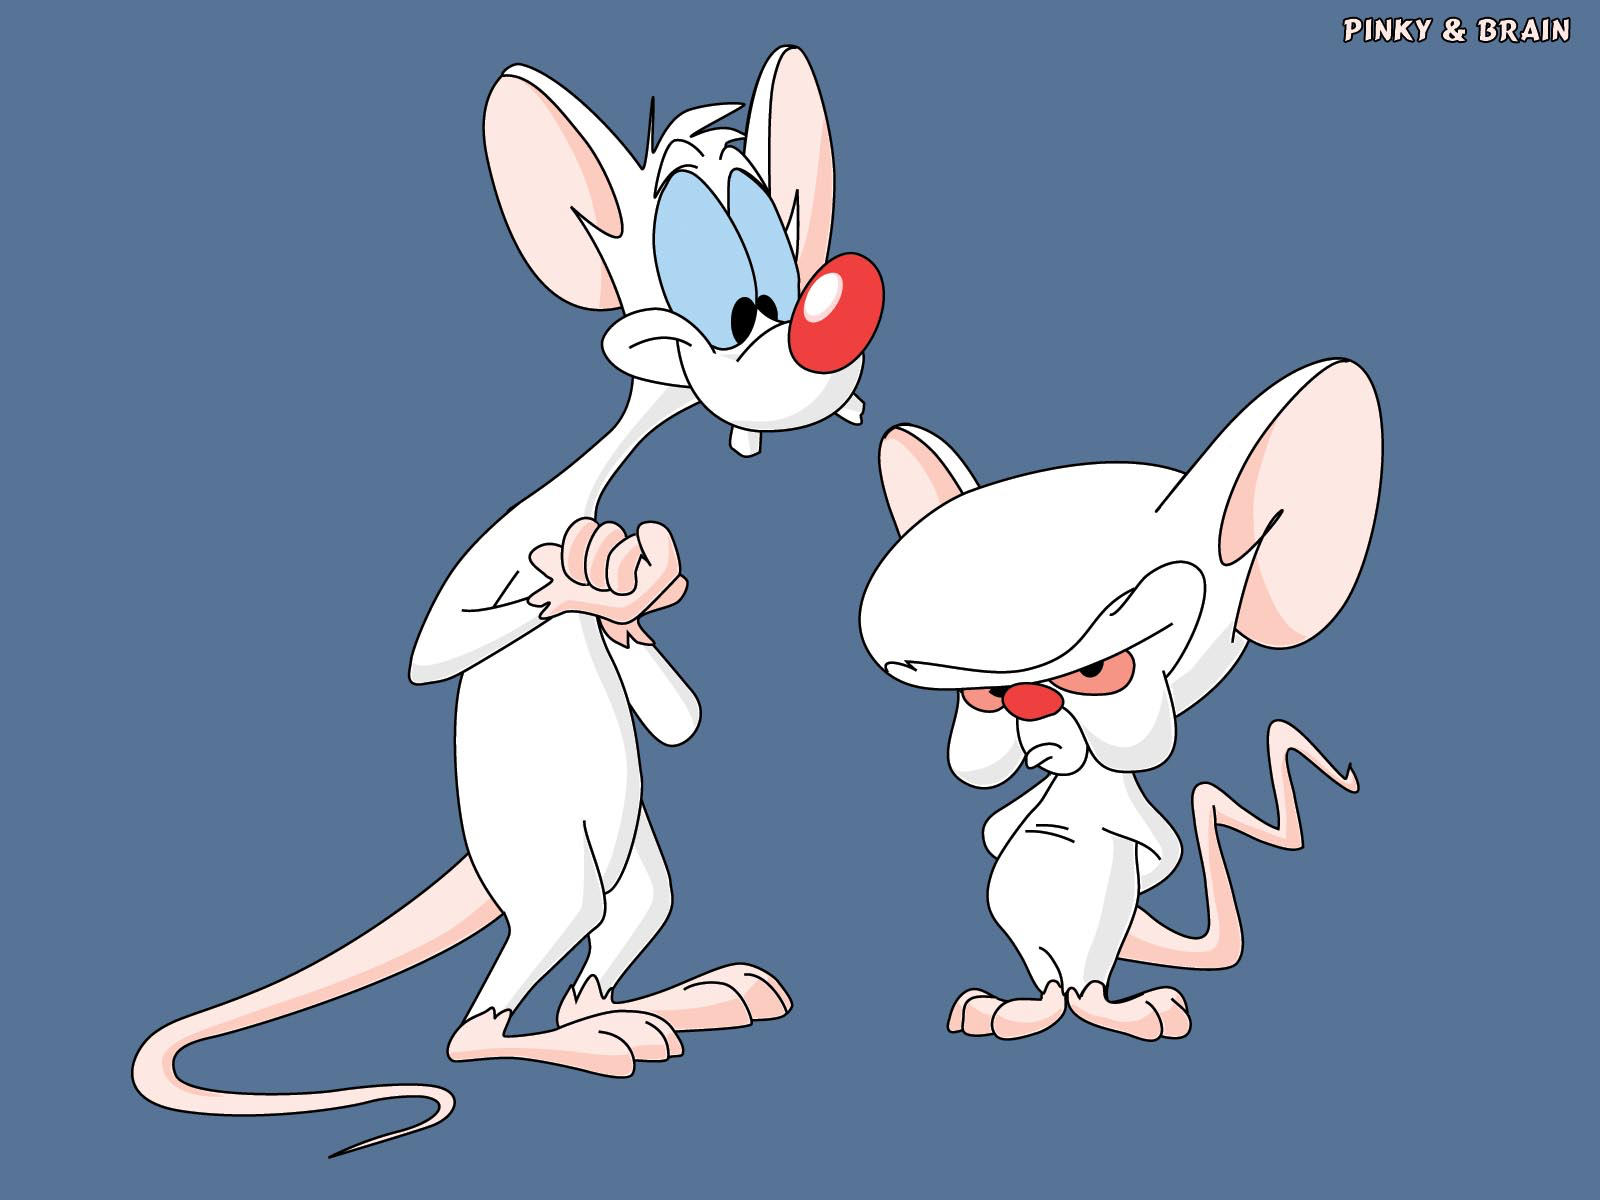
\includegraphics[scale=0.5]{./img/pinky-and-the-brain.png}
\caption{Etymology of Pinky's name.}
\label{fig:pinky-and-the-brain}
\end{center}
\end{figure}

\section{Overview of EEG Analysis}

TODO:
What is EEG analysis? Why is it important? What is the scale of the problem? How have we fixed it?

\section{System Architecture}

The system is comprised of three coupled layers which handle, storage,
computation and visualization. Figure \ref{fig:system-architecture} shows the
overall architecture of the system.

\begin{figure}[h]
\begin{center}
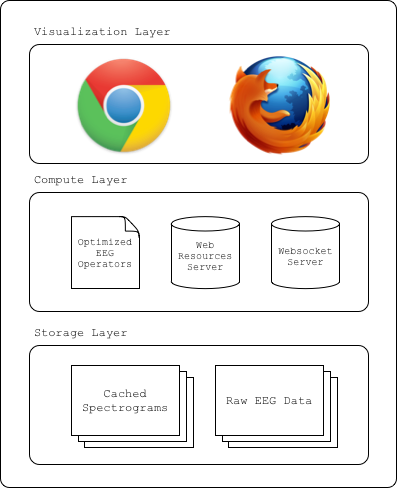
\includegraphics[scale=0.75]{./img/system-architecture.png}
\caption{Pinky System Architecture.}
\label{fig:system-architecture}
\end{center}
\end{figure}

\subsection{Storage Layer}

The storage layer, discuss in detail in chapter \ref{storage-ch}, is responsible for
storing raw EEG patient data and a copy of the calculated spectrogram. This
datastore must be optimized for both reads and writes of array based data for
multidimensional arrays on the order to tens to hundreds of GB.

\subsection{Compute Layer}

The compute layer, discuss in detail in chapter \ref{compute-ch}, is meant to be an
extendible module which handles the algorithms to calculate the spectrogram and
other EEG related calculations. As we discuss in \ref{discuss-ch:future-work},
there are several extensions the project can take, thus it is important that an
interested developer can easily add functionality to this layer. In addition,
the compute layer contains two servers, one to server the array based data,
interfacing with the optimized EEG algorithms, and a lightweight server for the
web resources to be served to the visualization layer.

\subsection{Visualization Layer}

The visualization layer, discussed in detail in chapter \ref{viz-ch}, is a browser
based module that renders the data to the client. The interface allows users to
query based on a patient's id (medical record number, \c{mrn}) and view a spectrogram
for a given time interval.

\subsection{Visgoth System}

Since enabling interactivity is an important design criteria, we have designed
and built a optimization module for time series visualization in the browser,
Visgoth. This is discussed in detail in chapter \ref{visgoth-ch}.

\section{Usage}

The project code base is available publicly on Github \cite{github}
\url{https://github.com/joshblum/eeg-toolkit} with documentation for installing
the project for development. In addition, we have created Docker \cite{docker}
images that can easily be install for production use. Armed with a dataset, any
curious doctor should be able to install the images and load the data for
analysis. The docker images are available for public use here:
\url{https://hub.docker.com/r/joshblum/eeg-toolkit-webapp} and
\url{https://hub.docker.com/r/joshblum/eeg-toolkit-toolkit}. Specific
installation instructions can be found with the github project.

\section{Contributions}

Pinky make several contributions:

\begin{itemize}
  \item Implements an abstraction for array based storage systems.
  \item Implements 4 different backends to adhere to the abstraction.
  \item Evaluates the different backends for multiple input ranges and workloads.
  \item Implements optimized algorithms for analysing EEG data.
  \item Provides an extendible framework for accessing array based data and visualizing it in the browser.
  \item Implements scalable in-browser visualizations using the client's GPU.
  \item Implements a new system, Visgoth, for reducing latency for time series based visualizations.
\end{itemize}

These contributions enable doctors and medical expert analysts to interactively
analyse EEG data at scale.


\appendix
%% This defines the bibliography file (main.bib) and the bibliography style.
%% If you want to create a bibliography file by hand, change the contents of
%% this file to a `thebibliography' environment.  For more information 
%% see section 4.3 of the LaTeX manual.
\begin{singlespace}
\bibliography{main}
\bibliographystyle{plain}
\end{singlespace}

\end{document}

